\documentclass{standalone}
\usepackage{tikz}
\usetikzlibrary{patterns, positioning}
\usepackage[sfdefault]{ClearSans} %% option 'sfdefault' activates Clear Sans as the default text font
\usepackage[T1]{fontenc}

\begin{document}
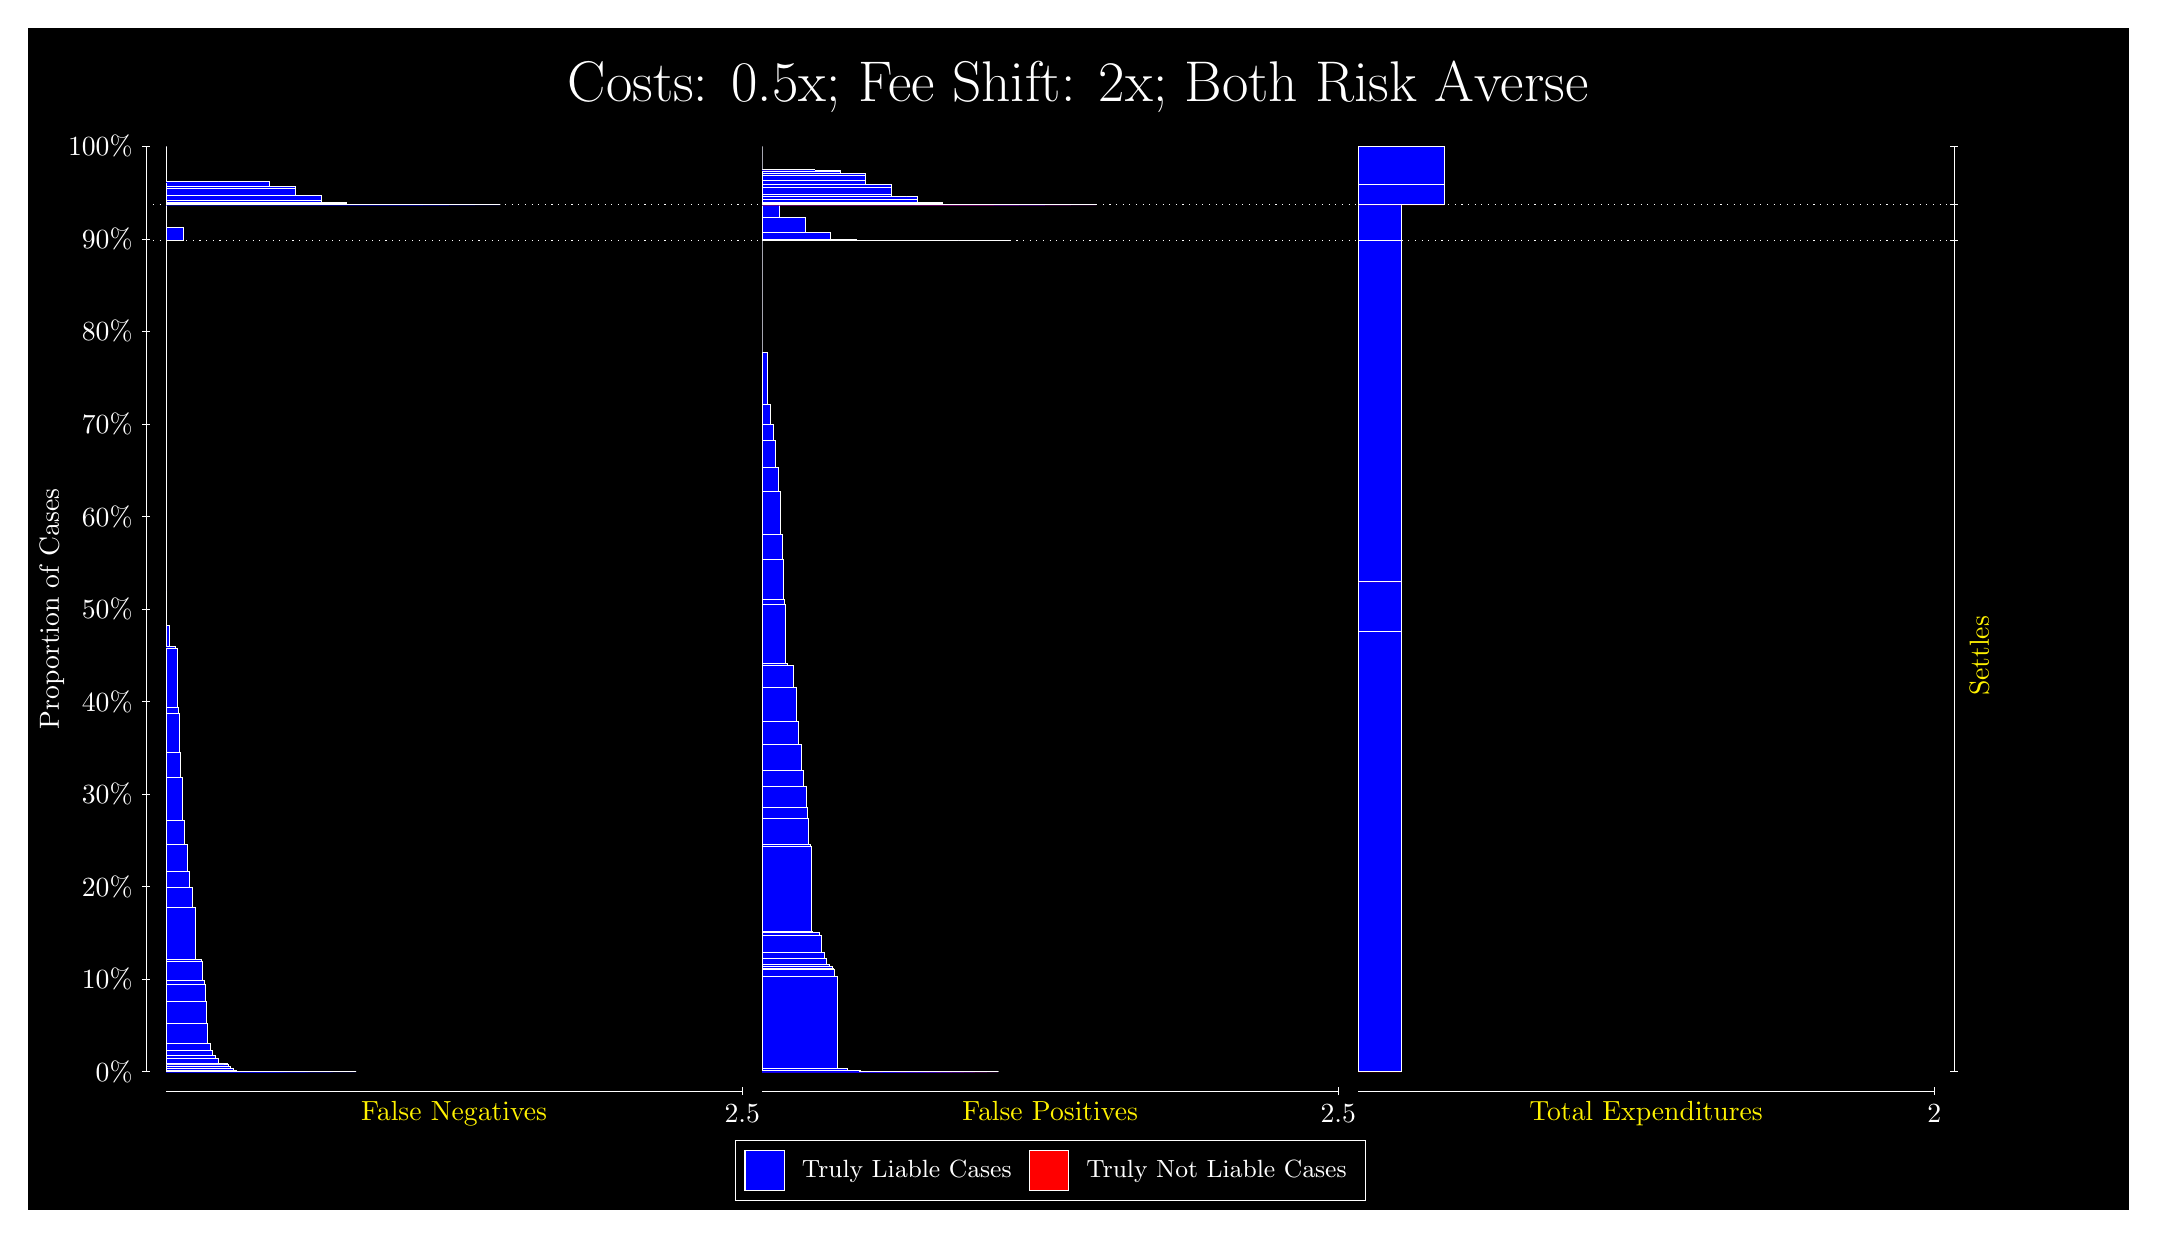
\begin{tikzpicture}
\draw[fill=black] (0,0) rectangle (26.667,15);
\draw[text=white] (0,13.5) rectangle (26.667,15) node[midway] {\huge Costs: 0.5x; Fee Shift: 2x; Both Risk Averse};
\draw[white, very thin] (1.5,1.75) -- (1.5,13.5);
\node[rotate=90, text=white, anchor=center] at (0.3, 7.625) {Proportion of Cases};
\draw[white, very thin] (1.45,1.75) -- (1.55,1.75);
\node[text=white, anchor=east] at (1.45, 1.75) {0\%};
\draw[white, very thin] (1.45,2.925) -- (1.55,2.925);
\node[text=white, anchor=east] at (1.45, 2.925) {10\%};
\draw[white, very thin] (1.45,4.1) -- (1.55,4.1);
\node[text=white, anchor=east] at (1.45, 4.1) {20\%};
\draw[white, very thin] (1.45,5.275) -- (1.55,5.275);
\node[text=white, anchor=east] at (1.45, 5.275) {30\%};
\draw[white, very thin] (1.45,6.45) -- (1.55,6.45);
\node[text=white, anchor=east] at (1.45, 6.45) {40\%};
\draw[white, very thin] (1.45,7.625) -- (1.55,7.625);
\node[text=white, anchor=east] at (1.45, 7.625) {50\%};
\draw[white, very thin] (1.45,8.8) -- (1.55,8.8);
\node[text=white, anchor=east] at (1.45, 8.8) {60\%};
\draw[white, very thin] (1.45,9.975) -- (1.55,9.975);
\node[text=white, anchor=east] at (1.45, 9.975) {70\%};
\draw[white, very thin] (1.45,11.15) -- (1.55,11.15);
\node[text=white, anchor=east] at (1.45, 11.15) {80\%};
\draw[white, very thin] (1.45,12.325) -- (1.55,12.325);
\node[text=white, anchor=east] at (1.45, 12.325) {90\%};
\draw[white, very thin] (1.45,13.5) -- (1.55,13.5);
\node[text=white, anchor=east] at (1.45, 13.5) {100\%};

\draw[white, very thin] (24.457,1.75) -- (24.457,13.5);
\draw[white, very thin] (24.407,1.75) -- (24.507,1.75);
\node[anchor=west] at (24.407, 1.75) {};
\draw[white, very thin] (24.407,12.307) -- (24.507,12.307);
\node[anchor=west] at (24.407, 12.307) {};
\draw[white, very thin] (24.407,12.761) -- (24.507,12.761);
\node[anchor=west] at (24.407, 12.761) {};
\draw[white, very thin] (24.407,13.5) -- (24.507,13.5);
\node[anchor=west] at (24.407, 13.5) {};

\draw[white, very thin, fill=blue] (1.75,1.75) rectangle (4.1652,1.75);
\draw[white, very thin, fill=blue] (1.75,1.75) rectangle (3.8725,1.75);
\draw[white, very thin, fill=blue] (1.75,1.75) rectangle (3.8399,1.75);
\draw[white, very thin, fill=blue] (1.75,1.75) rectangle (3.5797,1.75);
\draw[white, very thin, fill=blue] (1.75,1.75) rectangle (3.5472,1.75);
\draw[white, very thin, fill=blue] (1.75,1.75) rectangle (3.5147,1.75);
\draw[white, very thin, fill=blue] (1.75,1.75) rectangle (3.287,1.75);
\draw[white, very thin, fill=blue] (1.75,1.75) rectangle (3.2544,1.75);
\draw[white, very thin, fill=blue] (1.75,1.75) rectangle (3.2219,1.75);
\draw[white, very thin, fill=blue] (1.75,1.75) rectangle (3.1894,1.75);
\draw[white, very thin, fill=blue] (1.75,1.75) rectangle (3.1406,1.75);
\draw[white, very thin, fill=blue] (1.75,1.75) rectangle (2.9942,1.7501);
\draw[white, very thin, fill=blue] (1.75,1.7501) rectangle (2.9617,1.7501);
\draw[white, very thin, fill=blue] (1.75,1.7501) rectangle (2.9292,1.7506);
\draw[white, very thin, fill=blue] (1.75,1.7506) rectangle (2.8966,1.7511);
\draw[white, very thin, fill=blue] (1.75,1.7511) rectangle (2.8641,1.7516);
\draw[white, very thin, fill=blue] (1.75,1.7516) rectangle (2.8478,1.7519);
\draw[white, very thin, fill=blue] (1.75,1.7519) rectangle (2.8153,1.7519);
\draw[white, very thin, fill=blue] (1.75,1.7519) rectangle (2.7015,1.754);
\draw[white, very thin, fill=blue] (1.75,1.754) rectangle (2.6689,1.758);
\draw[white, very thin, fill=blue] (1.75,1.758) rectangle (2.6364,1.763);
\draw[white, very thin, fill=blue] (1.75,1.763) rectangle (2.6039,1.7884);
\draw[white, very thin, fill=blue] (1.75,1.7884) rectangle (2.5713,1.8121);
\draw[white, very thin, fill=blue] (1.75,1.8121) rectangle (2.5551,1.8202);
\draw[white, very thin, fill=blue] (1.75,1.8202) rectangle (2.5388,1.8445);
\draw[white, very thin, fill=blue] (1.75,1.8445) rectangle (2.5225,1.8487);
\draw[white, very thin, fill=blue] (1.75,1.8487) rectangle (2.49,1.8488);
\draw[white, very thin, fill=blue] (1.75,1.8488) rectangle (2.4087,1.9171);
\draw[white, very thin, fill=blue] (1.75,1.9171) rectangle (2.3762,1.9513);
\draw[white, very thin, fill=blue] (1.75,1.9513) rectangle (2.3436,2.024);
\draw[white, very thin, fill=blue] (1.75,2.024) rectangle (2.3111,2.1146);
\draw[white, very thin, fill=blue] (1.75,2.1146) rectangle (2.2786,2.3665);
\draw[white, very thin, fill=blue] (1.75,2.3665) rectangle (2.2623,2.6364);
\draw[white, very thin, fill=blue] (1.75,2.6364) rectangle (2.2461,2.8628);
\draw[white, very thin, fill=blue] (1.75,2.8628) rectangle (2.2298,2.9044);
\draw[white, very thin, fill=blue] (1.75,2.9044) rectangle (2.2135,3.155);
\draw[white, very thin, fill=blue] (1.75,3.155) rectangle (2.1973,3.1731);
\draw[white, very thin, fill=blue] (1.75,3.1731) rectangle (2.1647,3.1735);
\draw[white, very thin, fill=blue] (1.75,3.1735) rectangle (2.1159,3.8325);
\draw[white, very thin, fill=blue] (1.75,3.8325) rectangle (2.0834,4.0926);
\draw[white, very thin, fill=blue] (1.75,4.0926) rectangle (2.0509,4.2933);
\draw[white, very thin, fill=blue] (1.75,4.2933) rectangle (2.0184,4.6306);
\draw[white, very thin, fill=blue] (1.75,4.6306) rectangle (1.9858,4.9355);
\draw[white, very thin, fill=blue] (1.75,4.9355) rectangle (1.9533,5.4816);
\draw[white, very thin, fill=blue] (1.75,5.4816) rectangle (1.937,5.7982);
\draw[white, very thin, fill=blue] (1.75,5.7982) rectangle (1.9208,6.3058);
\draw[white, very thin, fill=blue] (1.75,6.3058) rectangle (1.9045,6.3717);
\draw[white, very thin, fill=blue] (1.75,6.3717) rectangle (1.8882,7.1275);
\draw[white, very thin, fill=blue] (1.75,7.1275) rectangle (1.872,7.1446);
\draw[white, very thin, fill=blue] (1.75,7.1446) rectangle (1.8395,7.145);
\draw[white, very thin, fill=blue] (1.75,7.145) rectangle (1.7907,7.4233);
\draw[white, very thin, fill=blue] (1.75,7.4233) rectangle (1.7581,7.8561);
\draw[white, very thin, fill=red] (1.75,7.8561) rectangle (1.75,7.8561);
\draw[white, very thin, fill=blue] (1.75,7.8561) rectangle (1.75,12.307);
\draw[white, very thin, fill=blue] (1.75,12.307) rectangle (1.9696,12.467);
\draw[white, very thin, fill=red] (1.75,12.467) rectangle (1.75,12.467);
\draw[white, very thin, fill=blue] (1.75,12.467) rectangle (1.75,12.761);
\draw[white, very thin, fill=blue] (1.75,12.761) rectangle (5.9949,12.761);
\draw[white, very thin, fill=blue] (1.75,12.761) rectangle (5.6697,12.761);
\draw[white, very thin, fill=blue] (1.75,12.761) rectangle (5.3444,12.761);
\draw[white, very thin, fill=blue] (1.75,12.761) rectangle (5.3444,12.761);
\draw[white, very thin, fill=blue] (1.75,12.761) rectangle (5.0191,12.761);
\draw[white, very thin, fill=blue] (1.75,12.761) rectangle (4.6938,12.762);
\draw[white, very thin, fill=blue] (1.75,12.762) rectangle (4.3685,12.767);
\draw[white, very thin, fill=blue] (1.75,12.767) rectangle (4.0432,12.777);
\draw[white, very thin, fill=blue] (1.75,12.777) rectangle (4.0432,12.793);
\draw[white, very thin, fill=blue] (1.75,12.793) rectangle (3.718,12.809);
\draw[white, very thin, fill=blue] (1.75,12.809) rectangle (3.718,12.874);
\draw[white, very thin, fill=blue] (1.75,12.874) rectangle (3.3927,12.964);
\draw[white, very thin, fill=blue] (1.75,12.964) rectangle (3.3927,12.994);
\draw[white, very thin, fill=blue] (1.75,12.994) rectangle (3.2626,12.994);
\draw[white, very thin, fill=blue] (1.75,12.994) rectangle (3.0674,13.05);
\draw[white, very thin, fill=blue] (1.75,13.05) rectangle (2.9373,13.05);
\draw[white, very thin, fill=blue] (1.75,13.05) rectangle (2.7421,13.051);
\draw[white, very thin, fill=blue] (1.75,13.051) rectangle (2.7421,13.054);
\draw[white, very thin, fill=blue] (1.75,13.054) rectangle (2.7421,13.057);
\draw[white, very thin, fill=blue] (1.75,13.057) rectangle (2.612,13.057);
\draw[white, very thin, fill=blue] (1.75,13.057) rectangle (2.612,13.057);
\draw[white, very thin, fill=blue] (1.75,13.057) rectangle (2.4168,13.057);
\draw[white, very thin, fill=blue] (1.75,13.057) rectangle (2.4168,13.057);
\draw[white, very thin, fill=blue] (1.75,13.057) rectangle (2.2867,13.057);
\draw[white, very thin, fill=blue] (1.75,13.057) rectangle (2.2867,13.057);
\draw[white, very thin, fill=blue] (1.75,13.057) rectangle (2.0915,13.057);
\draw[white, very thin, fill=blue] (1.75,13.057) rectangle (2.0915,13.057);
\draw[white, very thin, fill=blue] (1.75,13.057) rectangle (1.9614,13.058);
\draw[white, very thin, fill=blue] (1.75,13.058) rectangle (1.9614,13.06);
\draw[white, very thin, fill=blue] (1.75,13.06) rectangle (1.7663,13.06);
\draw[white, very thin, fill=blue] (1.75,13.06) rectangle (1.7663,13.06);
\draw[white, very thin, fill=red] (1.75,13.06) rectangle (1.75,13.06);
\draw[white, very thin, fill=blue] (1.75,13.06) rectangle (1.75,13.5);
\draw[white, very thin, fill=red] (9.3189,1.75) rectangle (12.32,1.75);
\draw[white, very thin, fill=blue] (9.3189,1.75) rectangle (12.32,1.75);
\draw[white, very thin, fill=red] (9.3189,1.75) rectangle (12.173,1.75);
\draw[white, very thin, fill=blue] (9.3189,1.75) rectangle (12.173,1.75);
\draw[white, very thin, fill=red] (9.3189,1.75) rectangle (12.027,1.75);
\draw[white, very thin, fill=blue] (9.3189,1.75) rectangle (12.027,1.75);
\draw[white, very thin, fill=blue] (9.3189,1.75) rectangle (11.994,1.75);
\draw[white, very thin, fill=red] (9.3189,1.75) rectangle (11.88,1.75);
\draw[white, very thin, fill=blue] (9.3189,1.75) rectangle (11.88,1.75);
\draw[white, very thin, fill=blue] (9.3189,1.75) rectangle (11.848,1.75);
\draw[white, very thin, fill=red] (9.3189,1.75) rectangle (11.734,1.75);
\draw[white, very thin, fill=blue] (9.3189,1.75) rectangle (11.734,1.75);
\draw[white, very thin, fill=blue] (9.3189,1.75) rectangle (11.702,1.75);
\draw[white, very thin, fill=blue] (9.3189,1.75) rectangle (11.669,1.75);
\draw[white, very thin, fill=red] (9.3189,1.75) rectangle (11.588,1.75);
\draw[white, very thin, fill=blue] (9.3189,1.75) rectangle (11.588,1.75);
\draw[white, very thin, fill=blue] (9.3189,1.75) rectangle (11.555,1.75);
\draw[white, very thin, fill=blue] (9.3189,1.75) rectangle (11.523,1.75);
\draw[white, very thin, fill=red] (9.3189,1.75) rectangle (11.441,1.75);
\draw[white, very thin, fill=blue] (9.3189,1.75) rectangle (11.441,1.75);
\draw[white, very thin, fill=blue] (9.3189,1.75) rectangle (11.409,1.75);
\draw[white, very thin, fill=blue] (9.3189,1.75) rectangle (11.376,1.75);
\draw[white, very thin, fill=blue] (9.3189,1.75) rectangle (11.344,1.75);
\draw[white, very thin, fill=red] (9.3189,1.75) rectangle (11.295,1.75);
\draw[white, very thin, fill=blue] (9.3189,1.75) rectangle (11.295,1.75);
\draw[white, very thin, fill=blue] (9.3189,1.75) rectangle (11.262,1.75);
\draw[white, very thin, fill=blue] (9.3189,1.75) rectangle (11.23,1.75);
\draw[white, very thin, fill=blue] (9.3189,1.75) rectangle (11.197,1.75);
\draw[white, very thin, fill=red] (9.3189,1.75) rectangle (11.149,1.75);
\draw[white, very thin, fill=blue] (9.3189,1.75) rectangle (11.149,1.75);
\draw[white, very thin, fill=blue] (9.3189,1.75) rectangle (11.116,1.75);
\draw[white, very thin, fill=blue] (9.3189,1.75) rectangle (11.084,1.75);
\draw[white, very thin, fill=blue] (9.3189,1.75) rectangle (11.051,1.75);
\draw[white, very thin, fill=blue] (9.3189,1.75) rectangle (11.018,1.75);
\draw[white, very thin, fill=blue] (9.3189,1.75) rectangle (10.97,1.75);
\draw[white, very thin, fill=blue] (9.3189,1.75) rectangle (10.937,1.75);
\draw[white, very thin, fill=blue] (9.3189,1.75) rectangle (10.905,1.75);
\draw[white, very thin, fill=blue] (9.3189,1.75) rectangle (10.872,1.75);
\draw[white, very thin, fill=red] (9.3189,1.75) rectangle (10.856,1.75);
\draw[white, very thin, fill=blue] (9.3189,1.75) rectangle (10.856,1.75);
\draw[white, very thin, fill=blue] (9.3189,1.75) rectangle (10.823,1.75);
\draw[white, very thin, fill=blue] (9.3189,1.75) rectangle (10.791,1.75);
\draw[white, very thin, fill=blue] (9.3189,1.75) rectangle (10.758,1.7501);
\draw[white, very thin, fill=blue] (9.3189,1.7501) rectangle (10.726,1.7506);
\draw[white, very thin, fill=blue] (9.3189,1.7506) rectangle (10.693,1.7506);
\draw[white, very thin, fill=blue] (9.3189,1.7506) rectangle (10.644,1.7506);
\draw[white, very thin, fill=blue] (9.3189,1.7506) rectangle (10.612,1.7506);
\draw[white, very thin, fill=blue] (9.3189,1.7506) rectangle (10.579,1.7506);
\draw[white, very thin, fill=red] (9.3189,1.7506) rectangle (10.563,1.7506);
\draw[white, very thin, fill=blue] (9.3189,1.7506) rectangle (10.563,1.7611);
\draw[white, very thin, fill=blue] (9.3189,1.7611) rectangle (10.547,1.7615);
\draw[white, very thin, fill=blue] (9.3189,1.7615) rectangle (10.531,1.7623);
\draw[white, very thin, fill=blue] (9.3189,1.7623) rectangle (10.498,1.763);
\draw[white, very thin, fill=blue] (9.3189,1.763) rectangle (10.465,1.7657);
\draw[white, very thin, fill=blue] (9.3189,1.7657) rectangle (10.433,1.7704);
\draw[white, very thin, fill=blue] (9.3189,1.7704) rectangle (10.4,1.7933);
\draw[white, very thin, fill=blue] (9.3189,1.7933) rectangle (10.368,1.7951);
\draw[white, very thin, fill=blue] (9.3189,1.7951) rectangle (10.319,1.7951);
\draw[white, very thin, fill=blue] (9.3189,1.7951) rectangle (10.287,1.7952);
\draw[white, very thin, fill=red] (9.3189,1.7952) rectangle (10.27,1.7952);
\draw[white, very thin, fill=blue] (9.3189,1.7952) rectangle (10.27,2.9593);
\draw[white, very thin, fill=blue] (9.3189,2.9593) rectangle (10.254,2.9605);
\draw[white, very thin, fill=blue] (9.3189,2.9605) rectangle (10.238,3.0438);
\draw[white, very thin, fill=blue] (9.3189,3.0438) rectangle (10.222,3.0595);
\draw[white, very thin, fill=blue] (9.3189,3.0595) rectangle (10.205,3.09);
\draw[white, very thin, fill=blue] (9.3189,3.09) rectangle (10.173,3.1166);
\draw[white, very thin, fill=blue] (9.3189,3.1166) rectangle (10.14,3.1827);
\draw[white, very thin, fill=blue] (9.3189,3.1827) rectangle (10.108,3.2691);
\draw[white, very thin, fill=blue] (9.3189,3.2691) rectangle (10.075,3.478);
\draw[white, very thin, fill=blue] (9.3189,3.478) rectangle (10.043,3.5227);
\draw[white, very thin, fill=blue] (9.3189,3.5227) rectangle (9.9938,3.5228);
\draw[white, very thin, fill=blue] (9.3189,3.5228) rectangle (9.9613,3.526);
\draw[white, very thin, fill=blue] (9.3189,3.526) rectangle (9.945,4.6096);
\draw[white, very thin, fill=blue] (9.3189,4.6096) rectangle (9.9288,4.6314);
\draw[white, very thin, fill=blue] (9.3189,4.6314) rectangle (9.9125,4.9648);
\draw[white, very thin, fill=blue] (9.3189,4.9648) rectangle (9.8962,5.107);
\draw[white, very thin, fill=blue] (9.3189,5.107) rectangle (9.88,5.3782);
\draw[white, very thin, fill=blue] (9.3189,5.3782) rectangle (9.8475,5.5798);
\draw[white, very thin, fill=blue] (9.3189,5.5798) rectangle (9.8149,5.9118);
\draw[white, very thin, fill=blue] (9.3189,5.9118) rectangle (9.7824,6.2012);
\draw[white, very thin, fill=blue] (9.3189,6.2012) rectangle (9.7499,6.6341);
\draw[white, very thin, fill=blue] (9.3189,6.6341) rectangle (9.7173,6.9124);
\draw[white, very thin, fill=blue] (9.3189,6.9124) rectangle (9.6685,6.9127);
\draw[white, very thin, fill=blue] (9.3189,6.9127) rectangle (9.636,6.9299);
\draw[white, very thin, fill=blue] (9.3189,6.9299) rectangle (9.6198,7.6856);
\draw[white, very thin, fill=blue] (9.3189,7.6856) rectangle (9.6035,7.7515);
\draw[white, very thin, fill=blue] (9.3189,7.7515) rectangle (9.5872,8.2591);
\draw[white, very thin, fill=blue] (9.3189,8.2591) rectangle (9.571,8.5757);
\draw[white, very thin, fill=blue] (9.3189,8.5757) rectangle (9.5547,9.1218);
\draw[white, very thin, fill=blue] (9.3189,9.1218) rectangle (9.5222,9.4267);
\draw[white, very thin, fill=blue] (9.3189,9.4267) rectangle (9.4896,9.764);
\draw[white, very thin, fill=blue] (9.3189,9.764) rectangle (9.4571,9.9647);
\draw[white, very thin, fill=blue] (9.3189,9.9647) rectangle (9.4246,10.225);
\draw[white, very thin, fill=blue] (9.3189,10.225) rectangle (9.3921,10.884);
\draw[white, very thin, fill=blue] (9.3189,10.884) rectangle (9.3433,10.884);
\draw[white, very thin, fill=blue] (9.3189,10.884) rectangle (9.3189,12.307);
\draw[white, very thin, fill=red] (9.3189,12.307) rectangle (12.466,12.307);
\draw[white, very thin, fill=blue] (9.3189,12.307) rectangle (12.466,12.307);
\draw[white, very thin, fill=blue] (9.3189,12.307) rectangle (12.141,12.307);
\draw[white, very thin, fill=blue] (9.3189,12.307) rectangle (11.815,12.307);
\draw[white, very thin, fill=blue] (9.3189,12.307) rectangle (11.49,12.307);
\draw[white, very thin, fill=blue] (9.3189,12.307) rectangle (11.165,12.307);
\draw[white, very thin, fill=blue] (9.3189,12.307) rectangle (10.84,12.308);
\draw[white, very thin, fill=blue] (9.3189,12.308) rectangle (10.514,12.317);
\draw[white, very thin, fill=blue] (9.3189,12.317) rectangle (10.189,12.406);
\draw[white, very thin, fill=blue] (9.3189,12.406) rectangle (9.8637,12.602);
\draw[white, very thin, fill=blue] (9.3189,12.602) rectangle (9.5384,12.761);
\draw[white, very thin, fill=red] (9.3189,12.761) rectangle (13.564,12.761);
\draw[white, very thin, fill=blue] (9.3189,12.761) rectangle (13.564,12.761);
\draw[white, very thin, fill=red] (9.3189,12.761) rectangle (13.239,12.761);
\draw[white, very thin, fill=blue] (9.3189,12.761) rectangle (13.239,12.761);
\draw[white, very thin, fill=red] (9.3189,12.761) rectangle (12.913,12.761);
\draw[white, very thin, fill=blue] (9.3189,12.761) rectangle (12.913,12.761);
\draw[white, very thin, fill=blue] (9.3189,12.761) rectangle (12.913,12.761);
\draw[white, very thin, fill=red] (9.3189,12.761) rectangle (12.588,12.761);
\draw[white, very thin, fill=blue] (9.3189,12.761) rectangle (12.588,12.761);
\draw[white, very thin, fill=red] (9.3189,12.761) rectangle (12.263,12.761);
\draw[white, very thin, fill=blue] (9.3189,12.761) rectangle (12.263,12.762);
\draw[white, very thin, fill=blue] (9.3189,12.762) rectangle (11.937,12.763);
\draw[white, very thin, fill=blue] (9.3189,12.763) rectangle (11.937,12.763);
\draw[white, very thin, fill=red] (9.3189,12.763) rectangle (11.937,12.763);
\draw[white, very thin, fill=blue] (9.3189,12.763) rectangle (11.937,12.766);
\draw[white, very thin, fill=blue] (9.3189,12.766) rectangle (11.612,12.774);
\draw[white, very thin, fill=blue] (9.3189,12.774) rectangle (11.612,12.782);
\draw[white, very thin, fill=red] (9.3189,12.782) rectangle (11.612,12.782);
\draw[white, very thin, fill=blue] (9.3189,12.782) rectangle (11.612,12.788);
\draw[white, very thin, fill=blue] (9.3189,12.788) rectangle (11.287,12.829);
\draw[white, very thin, fill=blue] (9.3189,12.829) rectangle (11.287,12.865);
\draw[white, very thin, fill=blue] (9.3189,12.865) rectangle (11.287,12.866);
\draw[white, very thin, fill=red] (9.3189,12.866) rectangle (11.157,12.866);
\draw[white, very thin, fill=blue] (9.3189,12.866) rectangle (11.157,12.866);
\draw[white, very thin, fill=blue] (9.3189,12.866) rectangle (10.962,12.896);
\draw[white, very thin, fill=blue] (9.3189,12.896) rectangle (10.962,12.983);
\draw[white, very thin, fill=blue] (9.3189,12.983) rectangle (10.962,13.018);
\draw[white, very thin, fill=red] (9.3189,13.018) rectangle (10.831,13.018);
\draw[white, very thin, fill=blue] (9.3189,13.018) rectangle (10.831,13.018);
\draw[white, very thin, fill=blue] (9.3189,13.018) rectangle (10.636,13.071);
\draw[white, very thin, fill=blue] (9.3189,13.071) rectangle (10.636,13.131);
\draw[white, very thin, fill=blue] (9.3189,13.131) rectangle (10.636,13.16);
\draw[white, very thin, fill=red] (9.3189,13.16) rectangle (10.506,13.16);
\draw[white, very thin, fill=blue] (9.3189,13.16) rectangle (10.506,13.16);
\draw[white, very thin, fill=blue] (9.3189,13.16) rectangle (10.506,13.16);
\draw[white, very thin, fill=blue] (9.3189,13.16) rectangle (10.311,13.162);
\draw[white, very thin, fill=blue] (9.3189,13.162) rectangle (10.311,13.186);
\draw[white, very thin, fill=blue] (9.3189,13.186) rectangle (10.311,13.202);
\draw[white, very thin, fill=blue] (9.3189,13.202) rectangle (10.181,13.202);
\draw[white, very thin, fill=red] (9.3189,13.202) rectangle (10.181,13.202);
\draw[white, very thin, fill=blue] (9.3189,13.202) rectangle (10.181,13.202);
\draw[white, very thin, fill=blue] (9.3189,13.202) rectangle (9.9857,13.203);
\draw[white, very thin, fill=blue] (9.3189,13.203) rectangle (9.9857,13.203);
\draw[white, very thin, fill=blue] (9.3189,13.203) rectangle (9.9857,13.204);
\draw[white, very thin, fill=blue] (9.3189,13.204) rectangle (9.8556,13.204);
\draw[white, very thin, fill=red] (9.3189,13.204) rectangle (9.8556,13.204);
\draw[white, very thin, fill=blue] (9.3189,13.204) rectangle (9.8556,13.204);
\draw[white, very thin, fill=blue] (9.3189,13.204) rectangle (9.8556,13.204);
\draw[white, very thin, fill=blue] (9.3189,13.204) rectangle (9.6604,13.204);
\draw[white, very thin, fill=blue] (9.3189,13.204) rectangle (9.6604,13.204);
\draw[white, very thin, fill=blue] (9.3189,13.204) rectangle (9.5303,13.204);
\draw[white, very thin, fill=red] (9.3189,13.204) rectangle (9.5303,13.204);
\draw[white, very thin, fill=blue] (9.3189,13.204) rectangle (9.5303,13.204);
\draw[white, very thin, fill=blue] (9.3189,13.204) rectangle (9.5303,13.204);
\draw[white, very thin, fill=blue] (9.3189,13.204) rectangle (9.3351,13.204);
\draw[white, very thin, fill=blue] (9.3189,13.204) rectangle (9.3351,13.204);
\draw[white, very thin, fill=red] (9.3189,13.204) rectangle (9.3189,13.204);
\draw[white, very thin, fill=blue] (9.3189,13.204) rectangle (9.3189,13.5);
\draw[white, very thin, fill=red] (16.888,1.75) rectangle (17.437,1.75);
\draw[white, very thin, fill=blue] (16.888,1.75) rectangle (17.437,7.3408);
\draw[white, very thin, fill=red] (16.888,7.3408) rectangle (17.437,7.3408);
\draw[white, very thin, fill=blue] (16.888,7.3408) rectangle (17.437,7.9702);
\draw[white, very thin, fill=red] (16.888,7.9702) rectangle (17.437,7.9702);
\draw[white, very thin, fill=blue] (16.888,7.9702) rectangle (17.437,12.307);
\draw[white, very thin, fill=red] (16.888,12.307) rectangle (17.437,12.307);
\draw[white, very thin, fill=blue] (16.888,12.307) rectangle (17.437,12.761);
\draw[white, very thin, fill=red] (16.888,12.761) rectangle (17.986,12.761);
\draw[white, very thin, fill=blue] (16.888,12.761) rectangle (17.986,13.023);
\draw[white, very thin, fill=red] (16.888,13.023) rectangle (17.986,13.023);
\draw[white, very thin, fill=blue] (16.888,13.023) rectangle (17.986,13.5);
\draw[white, dotted] (1.5,12.307) -- (24.457,12.307);
\draw[white, dotted] (1.5,12.761) -- (24.457,12.761);
\draw[white, very thin] (1.75,1.5) -- (9.0689,1.5);
\node[text=yellow, anchor=north] at (5.4094, 1.5) {False Negatives};
\draw[white, very thin] (9.0689,1.45) -- (9.0689,1.55);
\node[text=white, anchor=north] at (9.0689, 1.45) {2.5};

\draw[white, very thin] (9.3189,1.5) -- (16.638,1.5);
\node[text=yellow, anchor=north] at (12.978, 1.5) {False Positives};
\draw[white, very thin] (16.638,1.45) -- (16.638,1.55);
\node[text=white, anchor=north] at (16.638, 1.45) {2.5};

\draw[white, very thin] (16.888,1.5) -- (24.207,1.5);
\node[text=yellow, anchor=north] at (20.547, 1.5) {Total Expenditures};
\draw[white, very thin] (24.207,1.45) -- (24.207,1.55);
\node[text=white, anchor=north] at (24.207, 1.45) {2};

\node[text=yellow, centered, rotate=90] at (24.777, 7.0287) {Settles};



\draw (12.978300999999998,1.5) node[draw=none] (baseCoordinate) {};
\begin{scope}[align=center]
        \matrix[scale=0.5, draw=white, below=0.5cm of baseCoordinate, nodes={draw}, column sep=0.1cm]{
            \node[rectangle, draw, minimum width=0.5cm, minimum height=0.5cm, fill=blue] {}; &
            \node[draw=none, font=\small, text=white] (B) {Truly Liable Cases}; &
            \node[rectangle, draw, minimum width=0.5cm, minimum height=0.5cm, fill=red] {}; &
            \node[draw=none, font=\small, text=white] (B) {Truly Not Liable Cases}; \\
            };
\end{scope}

\end{tikzpicture}
\end{document}